
% Default to the notebook output style

    


% Inherit from the specified cell style.




    
\documentclass[11pt]{article}

    
    
    \usepackage[T1]{fontenc}
    % Nicer default font (+ math font) than Computer Modern for most use cases
    \usepackage{mathpazo}

    % Basic figure setup, for now with no caption control since it's done
    % automatically by Pandoc (which extracts ![](path) syntax from Markdown).
    \usepackage{graphicx}
    % We will generate all images so they have a width \maxwidth. This means
    % that they will get their normal width if they fit onto the page, but
    % are scaled down if they would overflow the margins.
    \makeatletter
    \def\maxwidth{\ifdim\Gin@nat@width>\linewidth\linewidth
    \else\Gin@nat@width\fi}
    \makeatother
    \let\Oldincludegraphics\includegraphics
    % Set max figure width to be 80% of text width, for now hardcoded.
    \renewcommand{\includegraphics}[1]{\Oldincludegraphics[width=.8\maxwidth]{#1}}
    % Ensure that by default, figures have no caption (until we provide a
    % proper Figure object with a Caption API and a way to capture that
    % in the conversion process - todo).
    \usepackage{caption}
    \DeclareCaptionLabelFormat{nolabel}{}
    \captionsetup{labelformat=nolabel}

    \usepackage{adjustbox} % Used to constrain images to a maximum size 
    \usepackage{xcolor} % Allow colors to be defined
    \usepackage{enumerate} % Needed for markdown enumerations to work
    \usepackage{geometry} % Used to adjust the document margins
    \usepackage{amsmath} % Equations
    \usepackage{amssymb} % Equations
    \usepackage{textcomp} % defines textquotesingle
    % Hack from http://tex.stackexchange.com/a/47451/13684:
    \AtBeginDocument{%
        \def\PYZsq{\textquotesingle}% Upright quotes in Pygmentized code
    }
    \usepackage{upquote} % Upright quotes for verbatim code
    \usepackage{eurosym} % defines \euro
    \usepackage[mathletters]{ucs} % Extended unicode (utf-8) support
    \usepackage[utf8x]{inputenc} % Allow utf-8 characters in the tex document
    \usepackage{fancyvrb} % verbatim replacement that allows latex
    \usepackage{grffile} % extends the file name processing of package graphics 
                         % to support a larger range 
    % The hyperref package gives us a pdf with properly built
    % internal navigation ('pdf bookmarks' for the table of contents,
    % internal cross-reference links, web links for URLs, etc.)
    \usepackage{hyperref}
    \usepackage{longtable} % longtable support required by pandoc >1.10
    \usepackage{booktabs}  % table support for pandoc > 1.12.2
    \usepackage[inline]{enumitem} % IRkernel/repr support (it uses the enumerate* environment)
    \usepackage[normalem]{ulem} % ulem is needed to support strikethroughs (\sout)
                                % normalem makes italics be italics, not underlines
    

    
    
    % Colors for the hyperref package
    \definecolor{urlcolor}{rgb}{0,.145,.698}
    \definecolor{linkcolor}{rgb}{.71,0.21,0.01}
    \definecolor{citecolor}{rgb}{.12,.54,.11}

    % ANSI colors
    \definecolor{ansi-black}{HTML}{3E424D}
    \definecolor{ansi-black-intense}{HTML}{282C36}
    \definecolor{ansi-red}{HTML}{E75C58}
    \definecolor{ansi-red-intense}{HTML}{B22B31}
    \definecolor{ansi-green}{HTML}{00A250}
    \definecolor{ansi-green-intense}{HTML}{007427}
    \definecolor{ansi-yellow}{HTML}{DDB62B}
    \definecolor{ansi-yellow-intense}{HTML}{B27D12}
    \definecolor{ansi-blue}{HTML}{208FFB}
    \definecolor{ansi-blue-intense}{HTML}{0065CA}
    \definecolor{ansi-magenta}{HTML}{D160C4}
    \definecolor{ansi-magenta-intense}{HTML}{A03196}
    \definecolor{ansi-cyan}{HTML}{60C6C8}
    \definecolor{ansi-cyan-intense}{HTML}{258F8F}
    \definecolor{ansi-white}{HTML}{C5C1B4}
    \definecolor{ansi-white-intense}{HTML}{A1A6B2}

    % commands and environments needed by pandoc snippets
    % extracted from the output of `pandoc -s`
    \providecommand{\tightlist}{%
      \setlength{\itemsep}{0pt}\setlength{\parskip}{0pt}}
    \DefineVerbatimEnvironment{Highlighting}{Verbatim}{commandchars=\\\{\}}
    % Add ',fontsize=\small' for more characters per line
    \newenvironment{Shaded}{}{}
    \newcommand{\KeywordTok}[1]{\textcolor[rgb]{0.00,0.44,0.13}{\textbf{{#1}}}}
    \newcommand{\DataTypeTok}[1]{\textcolor[rgb]{0.56,0.13,0.00}{{#1}}}
    \newcommand{\DecValTok}[1]{\textcolor[rgb]{0.25,0.63,0.44}{{#1}}}
    \newcommand{\BaseNTok}[1]{\textcolor[rgb]{0.25,0.63,0.44}{{#1}}}
    \newcommand{\FloatTok}[1]{\textcolor[rgb]{0.25,0.63,0.44}{{#1}}}
    \newcommand{\CharTok}[1]{\textcolor[rgb]{0.25,0.44,0.63}{{#1}}}
    \newcommand{\StringTok}[1]{\textcolor[rgb]{0.25,0.44,0.63}{{#1}}}
    \newcommand{\CommentTok}[1]{\textcolor[rgb]{0.38,0.63,0.69}{\textit{{#1}}}}
    \newcommand{\OtherTok}[1]{\textcolor[rgb]{0.00,0.44,0.13}{{#1}}}
    \newcommand{\AlertTok}[1]{\textcolor[rgb]{1.00,0.00,0.00}{\textbf{{#1}}}}
    \newcommand{\FunctionTok}[1]{\textcolor[rgb]{0.02,0.16,0.49}{{#1}}}
    \newcommand{\RegionMarkerTok}[1]{{#1}}
    \newcommand{\ErrorTok}[1]{\textcolor[rgb]{1.00,0.00,0.00}{\textbf{{#1}}}}
    \newcommand{\NormalTok}[1]{{#1}}
    
    % Additional commands for more recent versions of Pandoc
    \newcommand{\ConstantTok}[1]{\textcolor[rgb]{0.53,0.00,0.00}{{#1}}}
    \newcommand{\SpecialCharTok}[1]{\textcolor[rgb]{0.25,0.44,0.63}{{#1}}}
    \newcommand{\VerbatimStringTok}[1]{\textcolor[rgb]{0.25,0.44,0.63}{{#1}}}
    \newcommand{\SpecialStringTok}[1]{\textcolor[rgb]{0.73,0.40,0.53}{{#1}}}
    \newcommand{\ImportTok}[1]{{#1}}
    \newcommand{\DocumentationTok}[1]{\textcolor[rgb]{0.73,0.13,0.13}{\textit{{#1}}}}
    \newcommand{\AnnotationTok}[1]{\textcolor[rgb]{0.38,0.63,0.69}{\textbf{\textit{{#1}}}}}
    \newcommand{\CommentVarTok}[1]{\textcolor[rgb]{0.38,0.63,0.69}{\textbf{\textit{{#1}}}}}
    \newcommand{\VariableTok}[1]{\textcolor[rgb]{0.10,0.09,0.49}{{#1}}}
    \newcommand{\ControlFlowTok}[1]{\textcolor[rgb]{0.00,0.44,0.13}{\textbf{{#1}}}}
    \newcommand{\OperatorTok}[1]{\textcolor[rgb]{0.40,0.40,0.40}{{#1}}}
    \newcommand{\BuiltInTok}[1]{{#1}}
    \newcommand{\ExtensionTok}[1]{{#1}}
    \newcommand{\PreprocessorTok}[1]{\textcolor[rgb]{0.74,0.48,0.00}{{#1}}}
    \newcommand{\AttributeTok}[1]{\textcolor[rgb]{0.49,0.56,0.16}{{#1}}}
    \newcommand{\InformationTok}[1]{\textcolor[rgb]{0.38,0.63,0.69}{\textbf{\textit{{#1}}}}}
    \newcommand{\WarningTok}[1]{\textcolor[rgb]{0.38,0.63,0.69}{\textbf{\textit{{#1}}}}}
    
    
    % Define a nice break command that doesn't care if a line doesn't already
    % exist.
    \def\br{\hspace*{\fill} \\* }
    % Math Jax compatability definitions
    \def\gt{>}
    \def\lt{<}
    % Document parameters
    \title{Romteknologi II - Hjemmeoppgaver}
    
    
    

    % Pygments definitions
    
\makeatletter
\def\PY@reset{\let\PY@it=\relax \let\PY@bf=\relax%
    \let\PY@ul=\relax \let\PY@tc=\relax%
    \let\PY@bc=\relax \let\PY@ff=\relax}
\def\PY@tok#1{\csname PY@tok@#1\endcsname}
\def\PY@toks#1+{\ifx\relax#1\empty\else%
    \PY@tok{#1}\expandafter\PY@toks\fi}
\def\PY@do#1{\PY@bc{\PY@tc{\PY@ul{%
    \PY@it{\PY@bf{\PY@ff{#1}}}}}}}
\def\PY#1#2{\PY@reset\PY@toks#1+\relax+\PY@do{#2}}

\expandafter\def\csname PY@tok@s\endcsname{\def\PY@tc##1{\textcolor[rgb]{0.73,0.13,0.13}{##1}}}
\expandafter\def\csname PY@tok@se\endcsname{\let\PY@bf=\textbf\def\PY@tc##1{\textcolor[rgb]{0.73,0.40,0.13}{##1}}}
\expandafter\def\csname PY@tok@gs\endcsname{\let\PY@bf=\textbf}
\expandafter\def\csname PY@tok@vc\endcsname{\def\PY@tc##1{\textcolor[rgb]{0.10,0.09,0.49}{##1}}}
\expandafter\def\csname PY@tok@s2\endcsname{\def\PY@tc##1{\textcolor[rgb]{0.73,0.13,0.13}{##1}}}
\expandafter\def\csname PY@tok@sx\endcsname{\def\PY@tc##1{\textcolor[rgb]{0.00,0.50,0.00}{##1}}}
\expandafter\def\csname PY@tok@gd\endcsname{\def\PY@tc##1{\textcolor[rgb]{0.63,0.00,0.00}{##1}}}
\expandafter\def\csname PY@tok@gr\endcsname{\def\PY@tc##1{\textcolor[rgb]{1.00,0.00,0.00}{##1}}}
\expandafter\def\csname PY@tok@il\endcsname{\def\PY@tc##1{\textcolor[rgb]{0.40,0.40,0.40}{##1}}}
\expandafter\def\csname PY@tok@cm\endcsname{\let\PY@it=\textit\def\PY@tc##1{\textcolor[rgb]{0.25,0.50,0.50}{##1}}}
\expandafter\def\csname PY@tok@nc\endcsname{\let\PY@bf=\textbf\def\PY@tc##1{\textcolor[rgb]{0.00,0.00,1.00}{##1}}}
\expandafter\def\csname PY@tok@vi\endcsname{\def\PY@tc##1{\textcolor[rgb]{0.10,0.09,0.49}{##1}}}
\expandafter\def\csname PY@tok@mh\endcsname{\def\PY@tc##1{\textcolor[rgb]{0.40,0.40,0.40}{##1}}}
\expandafter\def\csname PY@tok@s1\endcsname{\def\PY@tc##1{\textcolor[rgb]{0.73,0.13,0.13}{##1}}}
\expandafter\def\csname PY@tok@mi\endcsname{\def\PY@tc##1{\textcolor[rgb]{0.40,0.40,0.40}{##1}}}
\expandafter\def\csname PY@tok@ss\endcsname{\def\PY@tc##1{\textcolor[rgb]{0.10,0.09,0.49}{##1}}}
\expandafter\def\csname PY@tok@kd\endcsname{\let\PY@bf=\textbf\def\PY@tc##1{\textcolor[rgb]{0.00,0.50,0.00}{##1}}}
\expandafter\def\csname PY@tok@ch\endcsname{\let\PY@it=\textit\def\PY@tc##1{\textcolor[rgb]{0.25,0.50,0.50}{##1}}}
\expandafter\def\csname PY@tok@nv\endcsname{\def\PY@tc##1{\textcolor[rgb]{0.10,0.09,0.49}{##1}}}
\expandafter\def\csname PY@tok@gh\endcsname{\let\PY@bf=\textbf\def\PY@tc##1{\textcolor[rgb]{0.00,0.00,0.50}{##1}}}
\expandafter\def\csname PY@tok@sa\endcsname{\def\PY@tc##1{\textcolor[rgb]{0.73,0.13,0.13}{##1}}}
\expandafter\def\csname PY@tok@nt\endcsname{\let\PY@bf=\textbf\def\PY@tc##1{\textcolor[rgb]{0.00,0.50,0.00}{##1}}}
\expandafter\def\csname PY@tok@sh\endcsname{\def\PY@tc##1{\textcolor[rgb]{0.73,0.13,0.13}{##1}}}
\expandafter\def\csname PY@tok@gi\endcsname{\def\PY@tc##1{\textcolor[rgb]{0.00,0.63,0.00}{##1}}}
\expandafter\def\csname PY@tok@err\endcsname{\def\PY@bc##1{\setlength{\fboxsep}{0pt}\fcolorbox[rgb]{1.00,0.00,0.00}{1,1,1}{\strut ##1}}}
\expandafter\def\csname PY@tok@kr\endcsname{\let\PY@bf=\textbf\def\PY@tc##1{\textcolor[rgb]{0.00,0.50,0.00}{##1}}}
\expandafter\def\csname PY@tok@nn\endcsname{\let\PY@bf=\textbf\def\PY@tc##1{\textcolor[rgb]{0.00,0.00,1.00}{##1}}}
\expandafter\def\csname PY@tok@nb\endcsname{\def\PY@tc##1{\textcolor[rgb]{0.00,0.50,0.00}{##1}}}
\expandafter\def\csname PY@tok@c1\endcsname{\let\PY@it=\textit\def\PY@tc##1{\textcolor[rgb]{0.25,0.50,0.50}{##1}}}
\expandafter\def\csname PY@tok@vg\endcsname{\def\PY@tc##1{\textcolor[rgb]{0.10,0.09,0.49}{##1}}}
\expandafter\def\csname PY@tok@si\endcsname{\let\PY@bf=\textbf\def\PY@tc##1{\textcolor[rgb]{0.73,0.40,0.53}{##1}}}
\expandafter\def\csname PY@tok@gt\endcsname{\def\PY@tc##1{\textcolor[rgb]{0.00,0.27,0.87}{##1}}}
\expandafter\def\csname PY@tok@ow\endcsname{\let\PY@bf=\textbf\def\PY@tc##1{\textcolor[rgb]{0.67,0.13,1.00}{##1}}}
\expandafter\def\csname PY@tok@m\endcsname{\def\PY@tc##1{\textcolor[rgb]{0.40,0.40,0.40}{##1}}}
\expandafter\def\csname PY@tok@cpf\endcsname{\let\PY@it=\textit\def\PY@tc##1{\textcolor[rgb]{0.25,0.50,0.50}{##1}}}
\expandafter\def\csname PY@tok@w\endcsname{\def\PY@tc##1{\textcolor[rgb]{0.73,0.73,0.73}{##1}}}
\expandafter\def\csname PY@tok@fm\endcsname{\def\PY@tc##1{\textcolor[rgb]{0.00,0.00,1.00}{##1}}}
\expandafter\def\csname PY@tok@mo\endcsname{\def\PY@tc##1{\textcolor[rgb]{0.40,0.40,0.40}{##1}}}
\expandafter\def\csname PY@tok@c\endcsname{\let\PY@it=\textit\def\PY@tc##1{\textcolor[rgb]{0.25,0.50,0.50}{##1}}}
\expandafter\def\csname PY@tok@na\endcsname{\def\PY@tc##1{\textcolor[rgb]{0.49,0.56,0.16}{##1}}}
\expandafter\def\csname PY@tok@nd\endcsname{\def\PY@tc##1{\textcolor[rgb]{0.67,0.13,1.00}{##1}}}
\expandafter\def\csname PY@tok@k\endcsname{\let\PY@bf=\textbf\def\PY@tc##1{\textcolor[rgb]{0.00,0.50,0.00}{##1}}}
\expandafter\def\csname PY@tok@mb\endcsname{\def\PY@tc##1{\textcolor[rgb]{0.40,0.40,0.40}{##1}}}
\expandafter\def\csname PY@tok@ni\endcsname{\let\PY@bf=\textbf\def\PY@tc##1{\textcolor[rgb]{0.60,0.60,0.60}{##1}}}
\expandafter\def\csname PY@tok@kt\endcsname{\def\PY@tc##1{\textcolor[rgb]{0.69,0.00,0.25}{##1}}}
\expandafter\def\csname PY@tok@gp\endcsname{\let\PY@bf=\textbf\def\PY@tc##1{\textcolor[rgb]{0.00,0.00,0.50}{##1}}}
\expandafter\def\csname PY@tok@kn\endcsname{\let\PY@bf=\textbf\def\PY@tc##1{\textcolor[rgb]{0.00,0.50,0.00}{##1}}}
\expandafter\def\csname PY@tok@cp\endcsname{\def\PY@tc##1{\textcolor[rgb]{0.74,0.48,0.00}{##1}}}
\expandafter\def\csname PY@tok@nf\endcsname{\def\PY@tc##1{\textcolor[rgb]{0.00,0.00,1.00}{##1}}}
\expandafter\def\csname PY@tok@o\endcsname{\def\PY@tc##1{\textcolor[rgb]{0.40,0.40,0.40}{##1}}}
\expandafter\def\csname PY@tok@sr\endcsname{\def\PY@tc##1{\textcolor[rgb]{0.73,0.40,0.53}{##1}}}
\expandafter\def\csname PY@tok@ge\endcsname{\let\PY@it=\textit}
\expandafter\def\csname PY@tok@sc\endcsname{\def\PY@tc##1{\textcolor[rgb]{0.73,0.13,0.13}{##1}}}
\expandafter\def\csname PY@tok@gu\endcsname{\let\PY@bf=\textbf\def\PY@tc##1{\textcolor[rgb]{0.50,0.00,0.50}{##1}}}
\expandafter\def\csname PY@tok@kc\endcsname{\let\PY@bf=\textbf\def\PY@tc##1{\textcolor[rgb]{0.00,0.50,0.00}{##1}}}
\expandafter\def\csname PY@tok@no\endcsname{\def\PY@tc##1{\textcolor[rgb]{0.53,0.00,0.00}{##1}}}
\expandafter\def\csname PY@tok@go\endcsname{\def\PY@tc##1{\textcolor[rgb]{0.53,0.53,0.53}{##1}}}
\expandafter\def\csname PY@tok@kp\endcsname{\def\PY@tc##1{\textcolor[rgb]{0.00,0.50,0.00}{##1}}}
\expandafter\def\csname PY@tok@bp\endcsname{\def\PY@tc##1{\textcolor[rgb]{0.00,0.50,0.00}{##1}}}
\expandafter\def\csname PY@tok@vm\endcsname{\def\PY@tc##1{\textcolor[rgb]{0.10,0.09,0.49}{##1}}}
\expandafter\def\csname PY@tok@sb\endcsname{\def\PY@tc##1{\textcolor[rgb]{0.73,0.13,0.13}{##1}}}
\expandafter\def\csname PY@tok@ne\endcsname{\let\PY@bf=\textbf\def\PY@tc##1{\textcolor[rgb]{0.82,0.25,0.23}{##1}}}
\expandafter\def\csname PY@tok@dl\endcsname{\def\PY@tc##1{\textcolor[rgb]{0.73,0.13,0.13}{##1}}}
\expandafter\def\csname PY@tok@nl\endcsname{\def\PY@tc##1{\textcolor[rgb]{0.63,0.63,0.00}{##1}}}
\expandafter\def\csname PY@tok@mf\endcsname{\def\PY@tc##1{\textcolor[rgb]{0.40,0.40,0.40}{##1}}}
\expandafter\def\csname PY@tok@sd\endcsname{\let\PY@it=\textit\def\PY@tc##1{\textcolor[rgb]{0.73,0.13,0.13}{##1}}}
\expandafter\def\csname PY@tok@cs\endcsname{\let\PY@it=\textit\def\PY@tc##1{\textcolor[rgb]{0.25,0.50,0.50}{##1}}}

\def\PYZbs{\char`\\}
\def\PYZus{\char`\_}
\def\PYZob{\char`\{}
\def\PYZcb{\char`\}}
\def\PYZca{\char`\^}
\def\PYZam{\char`\&}
\def\PYZlt{\char`\<}
\def\PYZgt{\char`\>}
\def\PYZsh{\char`\#}
\def\PYZpc{\char`\%}
\def\PYZdl{\char`\$}
\def\PYZhy{\char`\-}
\def\PYZsq{\char`\'}
\def\PYZdq{\char`\"}
\def\PYZti{\char`\~}
% for compatibility with earlier versions
\def\PYZat{@}
\def\PYZlb{[}
\def\PYZrb{]}
\makeatother


    % Exact colors from NB
    \definecolor{incolor}{rgb}{0.0, 0.0, 0.5}
    \definecolor{outcolor}{rgb}{0.545, 0.0, 0.0}



    
    % Prevent overflowing lines due to hard-to-break entities
    \sloppy 
    % Setup hyperref package
    \hypersetup{
      breaklinks=true,  % so long urls are correctly broken across lines
      colorlinks=true,
      urlcolor=urlcolor,
      linkcolor=linkcolor,
      citecolor=citecolor,
      }
    % Slightly bigger margins than the latex defaults
    
    \geometry{verbose,tmargin=1in,bmargin=1in,lmargin=1in,rmargin=1in}
    
    

    \begin{document}
    
    
    \maketitle
    
    

    
    \section{Romteknologi II -
Hjemmeoppgaver}\label{romteknologi-ii---hjemmeoppgaver}

    \subsection{Oppgave 1}\label{oppgave-1}

    \begin{enumerate}
\def\labelenumi{\arabic{enumi}.}
\tightlist
\item
  Solen gjennomgår sykler på cirka 11 år. Gjennom grundig observasjon
  kan man forutsi når solen vil være på sitt mest, og minst aktive.
  Dette har konsekvenser for hvor mye stråling, og da også forstyrrelse
  som vil ramme Jorda. Generelt "romvær" er nyttig viten når man skal
  forvalte presise instrumenter plassert I baner og overgangsbaner.
\item
  Gjennom tidlig historie har stjerne- og spesielt solobservasjon latt
  sapiens forutsi årstider og andre klimatiske trender. Det er minst
  like sant den dag i dag, bare på mer detaljnivå.
\item
  Sola er en ganske gjennomsnittlig stjerne. Ved å observere den kan vi
  lære mye om stjerner generelt i rommet.
\end{enumerate}

    \subsection{Oppgave 2}\label{oppgave-2}

    \subsubsection{L1 Lagrange punkt}\label{l1-lagrange-punkt}

L1 er ett av totalt fem punkt hvor man finner balanse mellom to store
gravitasjonsbrønner. Som oftest snakker man om Jorda og Sola. I SOHO's
tilfelle er L1 det punktet innenfor Jorda, inn mot Sola. For å intuetivt
forstå punktet, kan man se for seg en balansegang. Nærme Jorda, faller
man mot Jorda, og nærme Sola, faller man mot Sola. Ett eller annet sted
I mellom, er det balanse og man faller i teorien ingensteder. Dette
kalles L1 og er 1.5x10\^{}6Km fra jordsentrum. Lagrangepunktene er i
praksis ikke helt stabile ettersom månen og andre påvirker banen. Derfor
må man i med noen få måneders mellomrom gjennopprette banen ved bruk av
noe drivstoff.

SOHO ble plassert her for å gi et uendrende perspektiv i Solas retning,
som er det samme som oss her på jorda.

\subsubsection{SOHO's oppdrag}\label{sohos-oppdrag}

SOHO's oppdrag var å studere Sola, men har siden også oppdaget over 3000
kometer. Den hadde tre hovedoppdag: 1. se på Solas yttre lag, herunder
coronaen samt opphavet til solvind 2. Studere egenskaper til L1 3. Prøve
å finne ut av Solas struktur.

    \subsection{Oppgave 3}\label{oppgave-3}

    Kommunikasjon med SOHO datt ut, og satellitten gikk inn i Emergency Sun
Reacquisition (ESR) mode. Den endte opp med en liten spinn og det tok
mange dager før man var i stand til å lokalisere og gjennnoppta
forbindelse med satellitten. Gjennom ren og skjær flaks tillot
rotasjonen noe sollys å treffe panelene i hver periode noe som tillot et
vågalt og suksserikt redningsforsøk i de påfølgende ukene. Alle 12
instrumenter for datasamling ble brukbare igjen, mens kontrollgyroene
aldri kom tilbake. Dette førte til en tidsperiode med dyre
rakettdytteaktiveringer (thruster burns) før ekspertgruppa var i stand
til å implimentere gyroløs kontroll 1.februar 1999 ved hjelp av
programvare. Denne teknikken var banebrytene og har senere inspirert
andre romfartøy.

    \subsection{Oppgave 4}\label{oppgave-4}

    Vi starter med å legge inn et par bibliotek som lar oss regne med
logaritmer og trigonometri, samt bruke benevning i fysiske størrelser

    \begin{Verbatim}[commandchars=\\\{\}]
{\color{incolor}In [{\color{incolor}1}]:} \PY{k+kn}{import} \PY{n+nn}{math}\PY{o}{,} \PY{n+nn}{physics}
\end{Verbatim}


    \begin{Verbatim}[commandchars=\\\{\}]
{\color{incolor}In [{\color{incolor}2}]:} \PY{k+kn}{from} \PY{n+nn}{physics} \PY{k}{import} \PY{n}{Q}
\end{Verbatim}


    \begin{Verbatim}[commandchars=\\\{\}]
{\color{incolor}In [{\color{incolor}3}]:} \PY{o}{\PYZpc{}}\PY{k}{load\PYZus{}ext} physics
\end{Verbatim}


    \begin{Verbatim}[commandchars=\\\{\}]
Unit calculation and physics extensions activated.

    \end{Verbatim}

    \begin{Verbatim}[commandchars=\\\{\}]
{\color{incolor}In [{\color{incolor}4}]:} \PY{n}{π}\PY{p}{,} \PY{n}{c} \PY{o}{=} \PY{n}{physics}\PY{o}{.}\PY{n}{\PYZus{}constants}\PY{p}{[}\PY{l+m+mi}{0}\PY{p}{]}\PY{p}{[}\PY{l+m+mi}{1}\PY{p}{]}\PY{p}{,} \PY{n}{physics}\PY{o}{.}\PY{n}{\PYZus{}constants}\PY{p}{[}\PY{l+m+mi}{2}\PY{p}{]}\PY{p}{[}\PY{l+m+mi}{1}\PY{p}{]} \PY{c+c1}{\PYZsh{} PI, Lysets hastighet i vakum}
\end{Verbatim}


    Først må vi legge inn verdiene og konvertere til SI

    \begin{Verbatim}[commandchars=\\\{\}]
{\color{incolor}In [{\color{incolor}5}]:} \PY{n}{f}\PY{p}{,} \PY{n}{D} \PY{o}{=} \PY{p}{(}\PY{l+m+mf}{2.25} \PY{n}{GHz}\PY{p}{)}\PY{o}{.}\PY{n}{base}\PY{p}{,} \PY{n}{Q}\PY{p}{(}\PY{l+m+mf}{1.5}\PY{o}{*}\PY{l+m+mi}{10}\PY{o}{*}\PY{o}{*}\PY{l+m+mi}{6}\PY{p}{,} \PY{l+s+s1}{\PYZsq{}}\PY{l+s+s1}{km}\PY{l+s+s1}{\PYZsq{}}\PY{p}{)}\PY{o}{.}\PY{n}{base} \PY{c+c1}{\PYZsh{} .base operatoren konverterer til SI hhv. Hz og m}
\end{Verbatim}


    \begin{Verbatim}[commandchars=\\\{\}]
{\color{incolor}In [{\color{incolor}6}]:} \PY{n}{λ} \PY{o}{=} \PY{n}{c}\PY{o}{/}\PY{n}{f}
\end{Verbatim}


    \begin{Verbatim}[commandchars=\\\{\}]
{\color{incolor}In [{\color{incolor}7}]:} \PY{n}{f}\PY{p}{,} \PY{n}{D}\PY{p}{,} \PY{n}{c}\PY{p}{,} \PY{n}{λ}
\end{Verbatim}


\begin{Verbatim}[commandchars=\\\{\}]
{\color{outcolor}Out[{\color{outcolor}7}]:} (2.25e+09 1/s, 1.5e+09 m, 2.9979246e+08 m/s, 0.13324109 m/1)
\end{Verbatim}
            
    Formelen for å regne ut \textbf{Free Space Loss} er: \textgreater{}
\(L_{0} = (\frac{4πD}{λ})^{2}\)

    \begin{Verbatim}[commandchars=\\\{\}]
{\color{incolor}In [{\color{incolor}8}]:} \PY{n}{L0} \PY{o}{=} \PY{p}{(}\PY{l+m+mi}{4}\PY{o}{*}\PY{n}{π}\PY{o}{*}\PY{n}{D}\PY{o}{/}\PY{n}{λ}\PY{p}{)}\PY{o}{*}\PY{o}{*}\PY{l+m+mi}{2}
\end{Verbatim}


    \begin{Verbatim}[commandchars=\\\{\}]
{\color{incolor}In [{\color{incolor}9}]:} \PY{n}{L0}
\end{Verbatim}


\begin{Verbatim}[commandchars=\\\{\}]
{\color{outcolor}Out[{\color{outcolor}9}]:} 2.0013630459705637e+22
\end{Verbatim}
            
    For å få \textbf{verdien i desibel} må vi ta: \textgreater{}
\(10 \times Log_{10}(Lineærverdi)\):

    \begin{Verbatim}[commandchars=\\\{\}]
{\color{incolor}In [{\color{incolor}10}]:} \PY{n}{L0\PYZus{}db} \PY{o}{=} \PY{l+m+mi}{10}\PY{o}{*}\PY{n}{math}\PY{o}{.}\PY{n}{log10}\PY{p}{(}\PY{n}{L0}\PY{p}{)}
\end{Verbatim}


    \begin{Verbatim}[commandchars=\\\{\}]
{\color{incolor}In [{\color{incolor}11}]:} \PY{n}{L0\PYZus{}db}
\end{Verbatim}


\begin{Verbatim}[commandchars=\\\{\}]
{\color{outcolor}Out[{\color{outcolor}11}]:} 223.01325876522426
\end{Verbatim}
            
    \begin{quote}
\subsubsection{\texorpdfstring{\textbf{Free Space Loss for SOHO er 223
dB}}{Free Space Loss for SOHO er 223 dB}}\label{free-space-loss-for-soho-er-223-db}
\end{quote}

    \subsection{Oppgave 5}\label{oppgave-5}

    Systemtemperatur har mye å si for radiostøy. Antennetemperatur er en
parameter som beskriver hvor mye støy en antenne produserer i et gitt
miljø. Dette kalles ofte antennesøty temperatur (antenna noise
temperature) og er ikke et mål på antennas fysiske temperatur. Derimot
avhenger den av dens \emph{"gain pattern"} og det termiske miljøet den
er utplassert i.

Opphavet er at temperaturen er en temperaturen er temperaturen på en
hypotesisk resistor med input av ideel \emph{"noise free receiver"} som
vil generere samme \emph{"output noise power per unit bandwidth"} som
antennen ved en spesifikk frekvens.

For å bedre signalet ønsker vi å redusere systemtemperaturen. Effekten
denne har er altså mer negativ ved høyere verdier.

    \subsection{Oppgave 6}\label{oppgave-6}

    Kort sagt, fordi satelliten ikke er akuratt i L1 og Sola er ekstremt mye
lenger unna satelitten enn det Jorda er.

Det lange svaret er at Sola er en enorm kilde til termnisk stråling og
radiostøy. Det vil si at strålespekteret utstrålt av Sola også dekker
båndet brukt av satellitten. En eksakt L1 posisjon ville altså vært
vannskelig å kommunisere med fordi for å peke en mottakerantenne på
jorda mot SOHO, måtte vi også pekt rett på Sola. Men om vi lar
satellitten ta en liten omvei rundt L1 unngår vi dette problemet. SOHO
er derfor ikke akuratt på L1, men i en såkalt Lissajous bane rundt den
som vist i figuren under. Denne banen har en periode på seks måneder,
mens rundt Sola går det naturligvis et år per periode.

\begin{figure}[htbp]
\centering
\includegraphics{http://images.slideplayer.com/25/7826609/slides/slide_6.jpg}
\caption{alt text}
\end{figure}

    \subsection{Oppgave 7}\label{oppgave-7}

    \subsection{Transmitter}\label{transmitter}

    Først noen ingangsverdier:

    \begin{Verbatim}[commandchars=\\\{\}]
{\color{incolor}In [{\color{incolor}12}]:} \PY{n}{Pt}\PY{p}{,} \PY{n}{antenna\PYZus{}diameter}\PY{p}{,} \PY{n}{antenna\PYZus{}efficiency} \PY{o}{=} \PY{n}{Q}\PY{p}{(}\PY{l+m+mf}{3.2}\PY{p}{,} \PY{l+s+s1}{\PYZsq{}}\PY{l+s+s1}{W}\PY{l+s+s1}{\PYZsq{}}\PY{p}{)}\PY{p}{,}  \PY{n}{Q}\PY{p}{(}\PY{l+m+mf}{0.8}\PY{p}{,} \PY{l+s+s1}{\PYZsq{}}\PY{l+s+s1}{m}\PY{l+s+s1}{\PYZsq{}}\PY{p}{)}\PY{p}{,} \PY{l+m+mf}{0.8} \PY{c+c1}{\PYZsh{} Pt er Transmitter power}
\end{Verbatim}


    \begin{Verbatim}[commandchars=\\\{\}]
{\color{incolor}In [{\color{incolor}13}]:} \PY{n}{A} \PY{o}{=} \PY{n}{π}\PY{o}{*}\PY{p}{(}\PY{n}{antenna\PYZus{}diameter}\PY{o}{/}\PY{l+m+mi}{2}\PY{p}{)}\PY{o}{*}\PY{o}{*}\PY{l+m+mi}{2} \PY{c+c1}{\PYZsh{} Aperture}
\end{Verbatim}


    \begin{Verbatim}[commandchars=\\\{\}]
{\color{incolor}In [{\color{incolor}14}]:} \PY{n}{Pt\PYZus{}db} \PY{o}{=} \PY{l+m+mi}{10}\PY{o}{*}\PY{n}{math}\PY{o}{.}\PY{n}{log10}\PY{p}{(}\PY{n}{Pt}\PY{o}{.}\PY{n}{value}\PY{p}{)} \PY{c+c1}{\PYZsh{} Omregnet til desibel}
\end{Verbatim}


    Formelen for å omregne \textbf{antenna gain} er: \textgreater{}
\(Gt = \frac{4πA}{λ^{2}}\)

    \begin{Verbatim}[commandchars=\\\{\}]
{\color{incolor}In [{\color{incolor}15}]:} \PY{n}{Gt} \PY{o}{=} \PY{n}{antenna\PYZus{}efficiency} \PY{o}{*} \PY{l+m+mi}{4}\PY{o}{*}\PY{n}{π}\PY{o}{*}\PY{n}{A}\PY{o}{/}\PY{n}{λ}\PY{o}{*}\PY{o}{*}\PY{l+m+mi}{2}
\end{Verbatim}


    \begin{Verbatim}[commandchars=\\\{\}]
{\color{incolor}In [{\color{incolor}16}]:} \PY{n}{Gt\PYZus{}db} \PY{o}{=} \PY{l+m+mi}{10}\PY{o}{*}\PY{n}{math}\PY{o}{.}\PY{n}{log10}\PY{p}{(}\PY{n}{Gt}\PY{p}{)}
\end{Verbatim}


    \begin{Verbatim}[commandchars=\\\{\}]
{\color{incolor}In [{\color{incolor}17}]:} \PY{n+nb}{print}\PY{p}{(}\PY{l+s+s1}{\PYZsq{}}\PY{l+s+s1}{Antenna gain i lineært: }\PY{l+s+s1}{\PYZsq{}} \PY{o}{+} \PY{n+nb}{str}\PY{p}{(}\PY{n}{Gt}\PY{p}{)} \PY{o}{+} \PY{l+s+s1}{\PYZsq{}}\PY{l+s+se}{\PYZbs{}n}\PY{l+s+s1}{Antenna gain i desibel: }\PY{l+s+s1}{\PYZsq{}} \PY{o}{+} \PY{n+nb}{str}\PY{p}{(}\PY{n}{Gt\PYZus{}db}\PY{p}{)} \PY{o}{+} \PY{l+s+s1}{\PYZsq{}}\PY{l+s+s1}{ db}\PY{l+s+s1}{\PYZsq{}}\PY{p}{)}
\end{Verbatim}


    \begin{Verbatim}[commandchars=\\\{\}]
Antenna gain i lineært: 284.6382998713691
Antenna gain i desibel: 24.542933367309683 db

    \end{Verbatim}

    Formelen for å regne ut \textbf{EiRP} er: \textgreater{}
\(Pt \times Gt\)

    \begin{Verbatim}[commandchars=\\\{\}]
{\color{incolor}In [{\color{incolor}18}]:} \PY{n}{EiRP} \PY{o}{=} \PY{n}{Pt} \PY{o}{*} \PY{n}{Gt}
\end{Verbatim}


    \begin{Verbatim}[commandchars=\\\{\}]
{\color{incolor}In [{\color{incolor}19}]:} \PY{n}{EiRP\PYZus{}db} \PY{o}{=} \PY{l+m+mi}{10}\PY{o}{*}\PY{n}{math}\PY{o}{.}\PY{n}{log10}\PY{p}{(}\PY{n}{EiRP}\PY{o}{.}\PY{n}{value}\PY{p}{)}
\end{Verbatim}


    \begin{Verbatim}[commandchars=\\\{\}]
{\color{incolor}In [{\color{incolor}20}]:} \PY{n+nb}{print}\PY{p}{(}\PY{l+s+s1}{\PYZsq{}}\PY{l+s+s1}{EiRP i lineært: }\PY{l+s+s1}{\PYZsq{}} \PY{o}{+} \PY{n+nb}{str}\PY{p}{(}\PY{n}{EiRP}\PY{p}{)} \PY{o}{+} \PY{l+s+s1}{\PYZsq{}}\PY{l+s+se}{\PYZbs{}n}\PY{l+s+s1}{EiRP i desibel: }\PY{l+s+s1}{\PYZsq{}} \PY{o}{+} \PY{n+nb}{str}\PY{p}{(}\PY{n}{EiRP\PYZus{}db}\PY{p}{)} \PY{o}{+} \PY{l+s+s1}{\PYZsq{}}\PY{l+s+s1}{ db}\PY{l+s+s1}{\PYZsq{}}\PY{p}{)}
\end{Verbatim}


    \begin{Verbatim}[commandchars=\\\{\}]
EiRP i lineært: 910.84256 W
EiRP i desibel: 29.594433150508745 db

    \end{Verbatim}

    \subsection{Receiver}\label{receiver}

    \begin{Verbatim}[commandchars=\\\{\}]
{\color{incolor}In [{\color{incolor}21}]:} \PY{n}{antenna\PYZus{}diameter}\PY{p}{,} \PY{n}{antenna\PYZus{}efficiency} \PY{o}{=} \PY{n}{Q}\PY{p}{(}\PY{l+m+mi}{26}\PY{p}{,} \PY{l+s+s1}{\PYZsq{}}\PY{l+s+s1}{m}\PY{l+s+s1}{\PYZsq{}}\PY{p}{)}\PY{p}{,}  \PY{l+m+mf}{0.9}
\end{Verbatim}


    \begin{Verbatim}[commandchars=\\\{\}]
{\color{incolor}In [{\color{incolor}22}]:} \PY{n}{A} \PY{o}{=} \PY{n}{π}\PY{o}{*}\PY{p}{(}\PY{n}{antenna\PYZus{}diameter}\PY{o}{/}\PY{l+m+mi}{2}\PY{p}{)}\PY{o}{*}\PY{o}{*}\PY{l+m+mi}{2} \PY{c+c1}{\PYZsh{} Aperture}
\end{Verbatim}


    Formelen for å regne ut \textbf{antenna gain} er: \textgreater{}
\(G_{r} = n \times \frac{4πA}{λ^{2}}\)

Hvor n er antenna efficiency og A er aperture

    \begin{Verbatim}[commandchars=\\\{\}]
{\color{incolor}In [{\color{incolor}23}]:} \PY{n}{Gr} \PY{o}{=} \PY{n}{antenna\PYZus{}efficiency} \PY{o}{*} \PY{l+m+mi}{4}\PY{o}{*}\PY{n}{π}\PY{o}{*}\PY{n}{A}\PY{o}{/}\PY{n}{λ}\PY{o}{*}\PY{o}{*}\PY{l+m+mi}{2}
\end{Verbatim}


    \begin{Verbatim}[commandchars=\\\{\}]
{\color{incolor}In [{\color{incolor}24}]:} \PY{n}{Gr\PYZus{}db} \PY{o}{=} \PY{l+m+mi}{10}\PY{o}{*}\PY{n}{math}\PY{o}{.}\PY{n}{log10}\PY{p}{(}\PY{n}{Gr}\PY{p}{)}
\end{Verbatim}


    \begin{Verbatim}[commandchars=\\\{\}]
{\color{incolor}In [{\color{incolor}25}]:} \PY{n+nb}{print}\PY{p}{(}\PY{l+s+s1}{\PYZsq{}}\PY{l+s+s1}{Antenna gain i lineært: }\PY{l+s+s1}{\PYZsq{}} \PY{o}{+} \PY{n+nb}{str}\PY{p}{(}\PY{n}{Gr}\PY{p}{)} \PY{o}{+} \PY{l+s+s1}{\PYZsq{}}\PY{l+s+se}{\PYZbs{}n}\PY{l+s+s1}{Antenna gain i desibel: }\PY{l+s+s1}{\PYZsq{}} \PY{o}{+} \PY{n+nb}{str}\PY{p}{(}\PY{n}{Gr\PYZus{}db}\PY{p}{)} \PY{o}{+} \PY{l+s+s1}{\PYZsq{}}\PY{l+s+s1}{ db}\PY{l+s+s1}{\PYZsq{}}\PY{p}{)}
\end{Verbatim}


    \begin{Verbatim}[commandchars=\\\{\}]
Antenna gain i lineært: 338230.3547690253
Antenna gain i desibel: 55.29212581136099 db

    \end{Verbatim}

    Formelen for \textbf{Recieved Power} er: \textgreater{}
\(P_{r} = \frac{EiRP \times G_{r} }{ L_{0}}\)

Alle verdier er i desibel.

    \begin{Verbatim}[commandchars=\\\{\}]
{\color{incolor}In [{\color{incolor}26}]:} \PY{n}{Pr\PYZus{}db} \PY{o}{=} \PY{n}{EiRP\PYZus{}db} \PY{o}{*} \PY{n}{Gr\PYZus{}db} \PY{o}{/} \PY{n}{L0\PYZus{}db}
\end{Verbatim}


    \begin{Verbatim}[commandchars=\\\{\}]
{\color{incolor}In [{\color{incolor}27}]:} \PY{n+nb}{print}\PY{p}{(}\PY{l+s+s1}{\PYZsq{}}\PY{l+s+s1}{Recieved Power er }\PY{l+s+s1}{\PYZsq{}} \PY{o}{+} \PY{n+nb}{str}\PY{p}{(}\PY{n}{Pr\PYZus{}db}\PY{p}{)} \PY{o}{+} \PY{l+s+s1}{\PYZsq{}}\PY{l+s+s1}{ dB}\PY{l+s+s1}{\PYZsq{}}\PY{p}{)}
\end{Verbatim}


    \begin{Verbatim}[commandchars=\\\{\}]
Recieved Power er 7.337407336827839 dB

    \end{Verbatim}

    For å gå videre å finne noise power density og carrier to noise ratio
trenger vi først å vite båndbredden. I slide 63 fra
Satellittkommunikasjonsforelesningen står det at:

\begin{itemize}
\tightlist
\item
  S/N = EsB/N0B
\item
  S/N er det samme som C/N
\item
  Da blir C/N0 = Es\emph{B/N0 = Eb}mB/N0
\end{itemize}

Vi kan da sette opp følgende uttrykk:

\begin{quote}
\(\frac{E_{b}mB}{N_{0}} = EiRP - L_{0} + \frac{Gr}{T} - k - B - L_{a}\)
\end{quote}

m er et mål for koding, og siden vi nå skal se bort i fra BPKS så antar
vi denne til 1. Den faller med andre ord bort. Hvis vi videre løser for
B får vi:

\begin{quote}
\(B = \frac{EiRP - L_{0} + \frac{Gr}{T} - k - L_{a}}{E_{b}/N_{0} + 1}\)
\end{quote}

Alle disse verdiene er kjent. Så nå gjenstår kun å legge inn
\(E_{b}/N_{0}\) og finne B:

    \begin{Verbatim}[commandchars=\\\{\}]
{\color{incolor}In [{\color{incolor}28}]:} \PY{n}{k}\PY{p}{,} \PY{n}{T} \PY{o}{=} \PY{n}{physics}\PY{o}{.}\PY{n}{\PYZus{}constants}\PY{p}{[}\PY{l+m+mi}{13}\PY{p}{]}\PY{p}{[}\PY{l+m+mi}{1}\PY{p}{]}\PY{p}{,} \PY{n}{Q}\PY{p}{(}\PY{l+m+mi}{78}\PY{p}{,} \PY{l+s+s1}{\PYZsq{}}\PY{l+s+s1}{K}\PY{l+s+s1}{\PYZsq{}}\PY{p}{)} \PY{c+c1}{\PYZsh{} boltzman\PYZsq{}s constant, Systemtemperatur}
\end{Verbatim}


    \begin{Verbatim}[commandchars=\\\{\}]
{\color{incolor}In [{\color{incolor}29}]:} \PY{n}{k\PYZus{}db}\PY{p}{,} \PY{n}{T\PYZus{}db}\PY{p}{,} \PY{n}{Eb\PYZus{}N0\PYZus{}db} \PY{o}{=} \PY{l+m+mi}{10}\PY{o}{*}\PY{n}{math}\PY{o}{.}\PY{n}{log10}\PY{p}{(}\PY{n}{k}\PY{o}{.}\PY{n}{value}\PY{p}{)}\PY{p}{,} \PY{l+m+mi}{10}\PY{o}{*}\PY{n}{math}\PY{o}{.}\PY{n}{log10}\PY{p}{(}\PY{n}{T}\PY{o}{.}\PY{n}{value}\PY{p}{)}\PY{p}{,} \PY{l+m+mi}{15}
\end{Verbatim}


    \begin{Verbatim}[commandchars=\\\{\}]
{\color{incolor}In [{\color{incolor}30}]:} \PY{n}{La\PYZus{}db} \PY{o}{=} \PY{l+m+mi}{10} \PY{c+c1}{\PYZsh{} Additional losses}
\end{Verbatim}


    \begin{Verbatim}[commandchars=\\\{\}]
{\color{incolor}In [{\color{incolor}31}]:} \PY{n}{B\PYZus{}db} \PY{o}{=} \PY{p}{(}\PY{n}{EiRP\PYZus{}db} \PY{o}{\PYZhy{}} \PY{n}{L0\PYZus{}db} \PY{o}{+} \PY{p}{(}\PY{n}{Gr\PYZus{}db}\PY{o}{/}\PY{n}{T\PYZus{}db}\PY{p}{)} \PY{o}{\PYZhy{}} \PY{n}{k\PYZus{}db} \PY{o}{\PYZhy{}} \PY{n}{La\PYZus{}db}\PY{p}{)} \PY{o}{/} \PY{p}{(}\PY{n}{Eb\PYZus{}N0\PYZus{}db} \PY{o}{+} \PY{l+m+mi}{1}\PY{p}{)}
\end{Verbatim}


    \begin{Verbatim}[commandchars=\\\{\}]
{\color{incolor}In [{\color{incolor}32}]:} \PY{n}{B} \PY{o}{=} \PY{n}{Q}\PY{p}{(}\PY{l+m+mi}{10}\PY{o}{*}\PY{o}{*}\PY{p}{(}\PY{n}{B\PYZus{}db}\PY{o}{/}\PY{l+m+mi}{10}\PY{p}{)}\PY{p}{,} \PY{l+s+s1}{\PYZsq{}}\PY{l+s+s1}{Hz}\PY{l+s+s1}{\PYZsq{}}\PY{p}{)} \PY{c+c1}{\PYZsh{} Omregner til lineært}
\end{Verbatim}


    \begin{Verbatim}[commandchars=\\\{\}]
{\color{incolor}In [{\color{incolor}33}]:} \PY{n}{B}\PY{p}{,} \PY{n}{B\PYZus{}db}
\end{Verbatim}


\begin{Verbatim}[commandchars=\\\{\}]
{\color{outcolor}Out[{\color{outcolor}33}]:} (1.4984468 Hz, 1.7564133042231056)
\end{Verbatim}
            
    Formelen for å regne ut \textbf{Noise power density} er: \textgreater{}
\(N = kTB\)

Hvor k er boltzman's konstant, T er systemtemperatur og B er båndbredden

    \begin{Verbatim}[commandchars=\\\{\}]
{\color{incolor}In [{\color{incolor}34}]:} \PY{n}{k}\PY{p}{,} \PY{n}{k\PYZus{}db}\PY{p}{,} \PY{n}{T}\PY{p}{,} \PY{n}{T\PYZus{}db}\PY{p}{,} \PY{n}{B}
\end{Verbatim}


\begin{Verbatim}[commandchars=\\\{\}]
{\color{outcolor}Out[{\color{outcolor}34}]:} (1.3806488e-23 J/K,
          -228.59916780233414,
          78 K,
          18.920946026904804,
          1.4984468 Hz)
\end{Verbatim}
            
    \begin{Verbatim}[commandchars=\\\{\}]
{\color{incolor}In [{\color{incolor}35}]:} \PY{n}{N} \PY{o}{=} \PY{n}{k} \PY{o}{*} \PY{n}{T} \PY{o}{*} \PY{n}{B} \PY{c+c1}{\PYZsh{} Noise power density}
\end{Verbatim}


    \begin{Verbatim}[commandchars=\\\{\}]
{\color{incolor}In [{\color{incolor}36}]:} \PY{n}{N\PYZus{}db} \PY{o}{=} \PY{l+m+mi}{10}\PY{o}{*}\PY{n}{math}\PY{o}{.}\PY{n}{log10}\PY{p}{(}\PY{n}{N}\PY{o}{.}\PY{n}{value}\PY{p}{)}
\end{Verbatim}


    \begin{Verbatim}[commandchars=\\\{\}]
{\color{incolor}In [{\color{incolor}37}]:} \PY{n}{N\PYZus{}db}
\end{Verbatim}


\begin{Verbatim}[commandchars=\\\{\}]
{\color{outcolor}Out[{\color{outcolor}37}]:} -207.92180847120622
\end{Verbatim}
            
    \textbf{Carrier to noise power density ratio C/N0} er det samme som
signal to noise ratio og regnes ut for desibel på følgende måte S/N\_db
= EiRP-L0 + G/T - k - B - La. Alle verdier er i desibel

    \begin{Verbatim}[commandchars=\\\{\}]
{\color{incolor}In [{\color{incolor}38}]:} \PY{n}{SNR\PYZus{}db} \PY{o}{=} \PY{n}{EiRP\PYZus{}db} \PY{o}{\PYZhy{}} \PY{n}{L0\PYZus{}db} \PY{o}{+} \PY{p}{(}\PY{n}{Gr\PYZus{}db}\PY{o}{/}\PY{n}{T\PYZus{}db}\PY{p}{)} \PY{o}{\PYZhy{}} \PY{n}{k\PYZus{}db} \PY{o}{\PYZhy{}} \PY{n}{B\PYZus{}db} \PY{o}{\PYZhy{}} \PY{n}{La\PYZus{}db} \PY{c+c1}{\PYZsh{} SNR er signal to noise ratio}
\end{Verbatim}


    \begin{Verbatim}[commandchars=\\\{\}]
{\color{incolor}In [{\color{incolor}39}]:} \PY{n}{SNR\PYZus{}db}
\end{Verbatim}


\begin{Verbatim}[commandchars=\\\{\}]
{\color{outcolor}Out[{\color{outcolor}39}]:} 26.346199563346588
\end{Verbatim}
            
    Når m = 1 så vil det si 1 bit / symbol, altså er båndbredde og
dataoverføringshastighet det samme. Vi får da en data\_rate lik B:

    \begin{Verbatim}[commandchars=\\\{\}]
{\color{incolor}In [{\color{incolor}40}]:} \PY{n}{data\PYZus{}rate} \PY{o}{=} \PY{n}{B}
\end{Verbatim}


    \begin{Verbatim}[commandchars=\\\{\}]
{\color{incolor}In [{\color{incolor}41}]:} \PY{n+nb}{print}\PY{p}{(}\PY{n+nb}{str}\PY{p}{(}\PY{n}{data\PYZus{}rate}\PY{o}{.}\PY{n}{value} \PY{o}{*} \PY{l+m+mi}{10}\PY{o}{*}\PY{o}{*}\PY{o}{\PYZhy{}}\PY{l+m+mi}{3}\PY{p}{)} \PY{o}{+} \PY{l+s+s1}{\PYZsq{}}\PY{l+s+s1}{ Mbit/s}\PY{l+s+s1}{\PYZsq{}}\PY{p}{)}
\end{Verbatim}


    \begin{Verbatim}[commandchars=\\\{\}]
0.0014984468062463137 Mbit/s

    \end{Verbatim}

    Vi får altså en overføringshastighet på 0.001 Mbit/s. Dette er utrolig
lavt, og stemmer sannsynligvis ikke.

    Oppgaven spør spesifikt om å besvare oppgaven ved å fylle ut excel
arket, så under følger det:

    \begin{figure}[htbp]
\centering
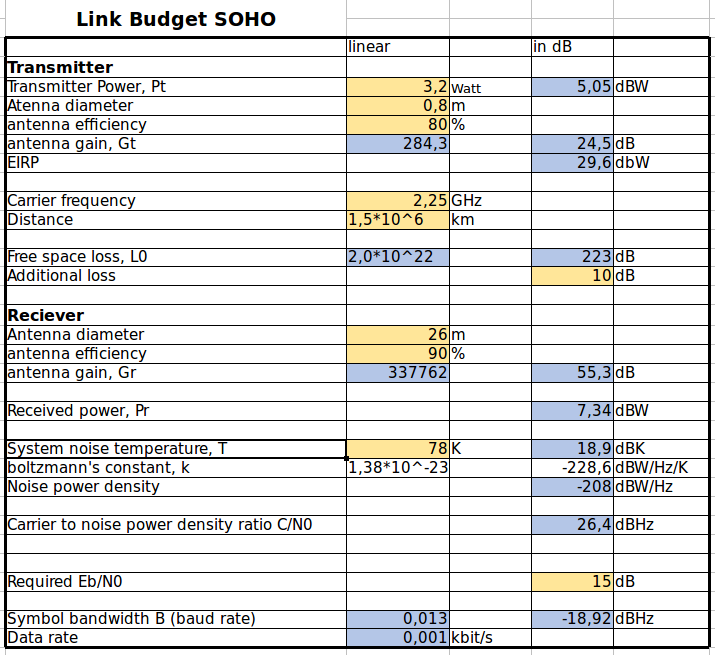
\includegraphics{img/space_tech/soho_excel.png}
\caption{soho\_excel}
\end{figure}

    \section{Oppgave 8}\label{oppgave-8}

    SDO står for Solar Dynamics Observatory. Målet til SDO satellitten er å
få en vitenskapelig forståelse for hvordan forbindelsen mellom Jorda og
Sola påvirker liv og samfund her på Jorda. Man ønsker også å se på
hvordan rommet nær Jorda blir påvirket av Solas nærvær. Videre studerer
SDO Solas magnetfelt og hvordan det påvirker solvind og andre
romvind-fenomener. Dette oppnåes blandt annet ved å studere mange
bølgelengder samtidig. Forskere prøver å bruke satellitten til å forstå
Solas magnetfelt oppstår og videre hvordan denne oppsamlede
magnetenergien slippes it i rommet i form av solvind og energi.

    \section{Oppgave 9}\label{oppgave-9}

    Banen til SDO er \emph{"inclined"} geostasjonær og satt til 102* Vest.
Denne banen er valgt for å gi kontinuerlig dekning av Sola samt relativt
høy overføringshastighet til kun én bakkestasjon. Et alternativ var LEO,
men dette ville ført til et behov for stor datalagringskapasitet. Man
gikk heller for en kontinuerlig forbindelse. Når man tar det valget, vil
det koste noe mer å skyte opp, da banen er lenger ut. Det vil også være
noen perioder med jordskygge og måneskygge vært år.

    \section{Oppgave 10}\label{oppgave-10}

    Likt som sist legger vi inn verdiene og konvertere til SI:

    \begin{Verbatim}[commandchars=\\\{\}]
{\color{incolor}In [{\color{incolor}42}]:} \PY{n}{f}\PY{p}{,} \PY{n}{D} \PY{o}{=} \PY{p}{(}\PY{l+m+mf}{26.5} \PY{n}{GHz}\PY{p}{)}\PY{o}{.}\PY{n}{base}\PY{p}{,} \PY{p}{(}\PY{l+m+mi}{35794} \PY{n}{km}\PY{p}{)}\PY{o}{.}\PY{n}{base}
\end{Verbatim}


    \begin{Verbatim}[commandchars=\\\{\}]
{\color{incolor}In [{\color{incolor}43}]:} \PY{n}{λ} \PY{o}{=} \PY{n}{c}\PY{o}{/}\PY{n}{f}
\end{Verbatim}


    \begin{Verbatim}[commandchars=\\\{\}]
{\color{incolor}In [{\color{incolor}44}]:} \PY{n}{L0} \PY{o}{=} \PY{p}{(}\PY{l+m+mi}{4}\PY{o}{*}\PY{n}{π}\PY{o}{*}\PY{n}{D}\PY{o}{/}\PY{n}{λ}\PY{p}{)}\PY{o}{*}\PY{o}{*}\PY{l+m+mi}{2}
\end{Verbatim}


    \begin{Verbatim}[commandchars=\\\{\}]
{\color{incolor}In [{\color{incolor}45}]:} \PY{n}{L0\PYZus{}db} \PY{o}{=} \PY{l+m+mi}{10}\PY{o}{*}\PY{n}{math}\PY{o}{.}\PY{n}{log10}\PY{p}{(}\PY{n}{L0}\PY{p}{)}
\end{Verbatim}


    \begin{Verbatim}[commandchars=\\\{\}]
{\color{incolor}In [{\color{incolor}46}]:} \PY{n}{f}\PY{p}{,} \PY{n}{D}\PY{p}{,} \PY{n}{c}\PY{p}{,} \PY{n}{λ}
\end{Verbatim}


\begin{Verbatim}[commandchars=\\\{\}]
{\color{outcolor}Out[{\color{outcolor}46}]:} (2.65e+10 1/s, 35794000 m, 2.9979246e+08 m/s, 0.011312923 m/1)
\end{Verbatim}
            
    \begin{Verbatim}[commandchars=\\\{\}]
{\color{incolor}In [{\color{incolor}47}]:} \PY{n}{L0\PYZus{}db}
\end{Verbatim}


\begin{Verbatim}[commandchars=\\\{\}]
{\color{outcolor}Out[{\color{outcolor}47}]:} 211.98890537580084
\end{Verbatim}
            
    \begin{quote}
\subsubsection{\texorpdfstring{\textbf{Free Space Loss for SDO er 212
dB}}{Free Space Loss for SDO er 212 dB}}\label{free-space-loss-for-sdo-er-212-db}
\end{quote}

    \section{Oppgave 11}\label{oppgave-11}

    Comment on the result compared to the data rate found from the SOHO
satellite

    \section{Polar Light}\label{polar-light}

\begin{center}\rule{0.5\linewidth}{\linethickness}\end{center}

    \section{Oppgave 12}\label{oppgave-12}

    \subsection{Trianguleringsmetoden}\label{trianguleringsmetoden}

    Trianguleringsmetoden som brukt til nordlysforskning går ut på å
observere og ta bilder fra forskjellige lokasjoner og deretter regne ut
høyde basert på observasjonsvinkelen. På figuren under kan man se
inngangsvariablene for en slik utregning der \emph{h} er den ukjente som
man ønsker å finne. 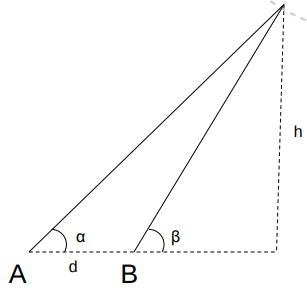
\includegraphics{img/space_tech/tri.png}

    \subsection{Utregning}\label{utregning}

    For å finne h må vi først finne x i trekanten ABC ved hjelp av
sinussetningen. I vårt tilfelle er vinklene som målingene er tatt med på
75 og 78 grader. Og de er tatt med 5 km mellomrom. Sinussetningen kan
lett regnes om til x = d * (sin∠B / sin∠C). Vinklene gir inngangsverdier
til å regne ut alle vinkler da vi vet at de til sammen er 180°:

    \begin{figure}[htbp]
\centering
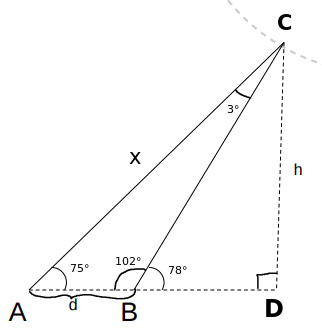
\includegraphics{img/space_tech/tri_math.png}
\caption{soho\_excel}
\end{figure}

    \begin{Verbatim}[commandchars=\\\{\}]
{\color{incolor}In [{\color{incolor}48}]:} \PY{n}{d}\PY{p}{,} \PY{n}{sinB}\PY{p}{,} \PY{n}{sinC} \PY{o}{=} \PY{n}{Q}\PY{p}{(}\PY{l+m+mi}{5}\PY{p}{,} \PY{l+s+s1}{\PYZsq{}}\PY{l+s+s1}{km}\PY{l+s+s1}{\PYZsq{}}\PY{p}{)}\PY{p}{,} \PY{n}{math}\PY{o}{.}\PY{n}{sin}\PY{p}{(}\PY{n}{math}\PY{o}{.}\PY{n}{radians}\PY{p}{(}\PY{l+m+mi}{102}\PY{p}{)}\PY{p}{)}\PY{p}{,} \PY{n}{math}\PY{o}{.}\PY{n}{sin}\PY{p}{(}\PY{n}{math}\PY{o}{.}\PY{n}{radians}\PY{p}{(}\PY{l+m+mi}{3}\PY{p}{)}\PY{p}{)}
\end{Verbatim}


    \begin{Verbatim}[commandchars=\\\{\}]
{\color{incolor}In [{\color{incolor}49}]:} \PY{n}{x} \PY{o}{=} \PY{n}{d} \PY{o}{*} \PY{p}{(}\PY{n}{sinB} \PY{o}{/} \PY{n}{sinC}\PY{p}{)}
\end{Verbatim}


    \begin{Verbatim}[commandchars=\\\{\}]
{\color{incolor}In [{\color{incolor}50}]:} \PY{n}{d}\PY{p}{,} \PY{n}{sinB}\PY{p}{,} \PY{n}{sinC}\PY{p}{,} \PY{n}{x}
\end{Verbatim}


\begin{Verbatim}[commandchars=\\\{\}]
{\color{outcolor}Out[{\color{outcolor}50}]:} (5 km, 0.9781476007338057, 0.052335956242943835, 93.448909 km)
\end{Verbatim}
            
    For så å regne ut høyden \emph{h} må vi bruke pytagoras i kjent stil for
trekanten ADC: \textgreater{}
\(sinA = \frac{mot}{hyp} \to mot = sinA \times hyp \to h = sinA \times x\)

    \begin{Verbatim}[commandchars=\\\{\}]
{\color{incolor}In [{\color{incolor}51}]:} \PY{n}{sinA} \PY{o}{=} \PY{n}{math}\PY{o}{.}\PY{n}{sin}\PY{p}{(}\PY{n}{math}\PY{o}{.}\PY{n}{radians}\PY{p}{(}\PY{l+m+mi}{75}\PY{p}{)}\PY{p}{)}
\end{Verbatim}


    \begin{Verbatim}[commandchars=\\\{\}]
{\color{incolor}In [{\color{incolor}52}]:} \PY{n}{h} \PY{o}{=} \PY{n}{sinA} \PY{o}{*} \PY{n}{x}
\end{Verbatim}


    \begin{Verbatim}[commandchars=\\\{\}]
{\color{incolor}In [{\color{incolor}53}]:} \PY{n}{h}
\end{Verbatim}


\begin{Verbatim}[commandchars=\\\{\}]
{\color{outcolor}Out[{\color{outcolor}53}]:} 90.264714 km
\end{Verbatim}
            
    \begin{quote}
\subsubsection{\texorpdfstring{\textbf{Nordlysets høyde er i følge
Størmes trianguleringsmetode 90.3 km over
jordoverflaten}}{Nordlysets høyde er i følge Størmes trianguleringsmetode 90.3 km over jordoverflaten}}\label{nordlysets-huxf8yde-er-i-fuxf8lge-stuxf8rmes-trianguleringsmetode-90.3-km-over-jordoverflaten}

Det vil også si at nordlyset er relativt lavt, da nordlys vanligvis
befinner seg mellom 100 km og 150 km over bakken. Gitt at Jorda er flat,
men denne antakelsen er rimelig når avstanden kun er 5 km. ***
\end{quote}

    \section{Oppgave 13}\label{oppgave-13}

    Såkalt protonlys skjer som en følge av at energiprotoner, \(H^{+}\),
penetrerer atmosfæren og påvirker lyset.

\(M + H^{+} → M^{+} + H^{*}\)

\(H^{*} → H + hf\)

\(M + H → H^{+} + M + e_{n}\)

Så lenge den gjenværende energien i protonet er over 36 eV, kan
prosessen gjentaes.

https://en.wikipedia.org/wiki/Proton\_emission

    \section{Oppgave 14}\label{oppgave-14}

    Ved 486.1 nm er lyset blågrønt og den elektroniske energien går fra n=4
til n=2. Den skifter altså to nivåer 4→2 og har en energiforskjell på
2.55 eV.

    \section{Oppgave 15}\label{oppgave-15}

    Farten er overført til fotoner. Dopler shift på Δf/f=0.01. Hvor Δf er
frekvensforskjellen pga dopler shift og f er frekvensen for det
utstrålte fotonet

Formelen for doppler shift er i følge
https://www4.uwsp.edu/physastr/kmenning/Astr311/Lect21.pdf :
\textgreater{} \(\frac{Δλ}{λ} = \frac{v}{c}\)

    \begin{Verbatim}[commandchars=\\\{\}]
{\color{incolor}In [{\color{incolor}54}]:} \PY{n}{doppler\PYZus{}shift} \PY{o}{=} \PY{l+m+mf}{0.01}
\end{Verbatim}


    Vi vet at bølgelengden er λ = 486.1 nm. Dette gir en rest frekvens:

    \begin{Verbatim}[commandchars=\\\{\}]
{\color{incolor}In [{\color{incolor}55}]:} \PY{n}{fr} \PY{o}{=} \PY{n}{Q}\PY{p}{(}\PY{l+m+mf}{486.1}\PY{p}{,} \PY{l+s+s1}{\PYZsq{}}\PY{l+s+s1}{nm}\PY{l+s+s1}{\PYZsq{}}\PY{p}{)}\PY{o}{.}\PY{n}{base} \PY{c+c1}{\PYZsh{} Rest frequency}
\end{Verbatim}


    Videre må vi regne om til bølgelengde:

    \begin{Verbatim}[commandchars=\\\{\}]
{\color{incolor}In [{\color{incolor}56}]:} \PY{n}{λ} \PY{o}{=} \PY{n}{c} \PY{o}{/} \PY{n}{fr}
\end{Verbatim}


    \begin{Verbatim}[commandchars=\\\{\}]
{\color{incolor}In [{\color{incolor}57}]:} \PY{n}{num1} \PY{o}{=} \PY{n}{doppler\PYZus{}shift} \PY{o}{*} \PY{n}{fr}
\end{Verbatim}


    \begin{Verbatim}[commandchars=\\\{\}]
{\color{incolor}In [{\color{incolor}58}]:} \PY{n}{λ}\PY{p}{,} \PY{n}{fr}\PY{p}{,} \PY{n}{num1}
\end{Verbatim}


\begin{Verbatim}[commandchars=\\\{\}]
{\color{outcolor}Out[{\color{outcolor}58}]:} (6.1673001e+14 1/s, 4.861e-07 m, 4.861e-09 m)
\end{Verbatim}
            
    \begin{Verbatim}[commandchars=\\\{\}]
{\color{incolor}In [{\color{incolor}59}]:} \PY{n}{v} \PY{o}{=} \PY{n}{c} \PY{o}{*} \PY{p}{(}\PY{n}{num1} \PY{o}{/} \PY{n}{fr}\PY{p}{)}
\end{Verbatim}


    \begin{Verbatim}[commandchars=\\\{\}]
{\color{incolor}In [{\color{incolor}60}]:} \PY{n}{v}
\end{Verbatim}


\begin{Verbatim}[commandchars=\\\{\}]
{\color{outcolor}Out[{\color{outcolor}60}]:} 2997924.6 m/s
\end{Verbatim}
            
    \begin{quote}
\subsubsection{Vi får en fart på nesten 3000
Km/s}\label{vi-fuxe5r-en-fart-puxe5-nesten-3000-kms}
\end{quote}

    Den relative farten regner vi enkelt ut

    \begin{Verbatim}[commandchars=\\\{\}]
{\color{incolor}In [{\color{incolor}61}]:} \PY{n}{relative\PYZus{}speed} \PY{o}{=} \PY{n}{v} \PY{o}{/} \PY{n}{c}
\end{Verbatim}


    \begin{Verbatim}[commandchars=\\\{\}]
{\color{incolor}In [{\color{incolor}62}]:} \PY{n}{relative\PYZus{}speed}
\end{Verbatim}


\begin{Verbatim}[commandchars=\\\{\}]
{\color{outcolor}Out[{\color{outcolor}62}]:} 0.01
\end{Verbatim}
            
    \begin{quote}
\subsubsection{Farten er ganske nøyaktig 1\% av lysets
hastighet}\label{farten-er-ganske-nuxf8yaktig-1-av-lysets-hastighet}
\end{quote}

    \section{Oppgave 16}\label{oppgave-16}

    Formelen for \textbf{kinetisk energi} er: \textgreater{}
\(E_{k} = \frac{mv^{2}}{2}\)

    \begin{Verbatim}[commandchars=\\\{\}]
{\color{incolor}In [{\color{incolor}63}]:} \PY{n}{mass\PYZus{}proton}\PY{p}{,} \PY{n}{e0} \PY{o}{=} \PY{n}{physics}\PY{o}{.}\PY{n}{\PYZus{}constants}\PY{p}{[}\PY{l+m+mi}{10}\PY{p}{]}\PY{p}{[}\PY{l+m+mi}{1}\PY{p}{]}\PY{p}{,} \PY{n}{physics}\PY{o}{.}\PY{n}{\PYZus{}constants}\PY{p}{[}\PY{l+m+mi}{8}\PY{p}{]}\PY{p}{[}\PY{l+m+mi}{1}\PY{p}{]}
\end{Verbatim}


    \begin{Verbatim}[commandchars=\\\{\}]
{\color{incolor}In [{\color{incolor}64}]:} \PY{n}{Ek} \PY{o}{=} \PY{p}{(}\PY{n}{mass\PYZus{}proton} \PY{o}{*} \PY{p}{(}\PY{n}{v}\PY{o}{*}\PY{o}{*}\PY{l+m+mi}{2}\PY{p}{)}\PY{p}{)} \PY{o}{/} \PY{l+m+mi}{2}
\end{Verbatim}


    \begin{Verbatim}[commandchars=\\\{\}]
{\color{incolor}In [{\color{incolor}65}]:} \PY{n}{Ek}\PY{o}{.}\PY{n}{convert}\PY{p}{(}\PY{l+s+s1}{\PYZsq{}}\PY{l+s+s1}{J}\PY{l+s+s1}{\PYZsq{}}\PY{p}{)}
\end{Verbatim}


    \begin{Verbatim}[commandchars=\\\{\}]
{\color{incolor}In [{\color{incolor}66}]:} \PY{n}{Ek}
\end{Verbatim}


\begin{Verbatim}[commandchars=\\\{\}]
{\color{outcolor}Out[{\color{outcolor}66}]:} 7.5163874e-15 J
\end{Verbatim}
            
    Den kinetiske energien er 7.5e-15 J

    \begin{Verbatim}[commandchars=\\\{\}]
{\color{incolor}In [{\color{incolor}67}]:} \PY{n}{Ek\PYZus{}eV} \PY{o}{=} \PY{n}{Ek} \PY{o}{*} \PY{n}{e0}
\end{Verbatim}


    \begin{Verbatim}[commandchars=\\\{\}]
{\color{incolor}In [{\color{incolor}68}]:} \PY{n}{Ek\PYZus{}eV}
\end{Verbatim}


\begin{Verbatim}[commandchars=\\\{\}]
{\color{outcolor}Out[{\color{outcolor}68}]:} 1.204258e-33 J*C
\end{Verbatim}
            
    Den kinetiske energien er eV 1.2e-33 noe som ikke er skadelig for
mennesker.

    physics plugin docs:
http://www.southampton.ac.uk/\textasciitilde{}fangohr/blog/physical-quantities-numerical-value-with-units-in-python.html
plugin for python 3: https://github.com/TheGrum/python3-physics LateX
math: https://en.wikibooks.org/wiki/LaTeX/Mathematics

    \begin{Verbatim}[commandchars=\\\{\}]
{\color{incolor}In [{\color{incolor}69}]:} \PY{n}{physics}\PY{o}{.}\PY{n}{\PYZus{}constants}
\end{Verbatim}


\begin{Verbatim}[commandchars=\\\{\}]
{\color{outcolor}Out[{\color{outcolor}69}]:} [('pi', 3.141592653589793),
          ('e', 2.718281828459045),
          ('c0', 2.9979246e+08 m/s),
          ('mu0', 1.2566371e-06 m*kg/A\^{}2/s\^{}2),
          ('eps0', 8.8541878e-12 A\^{}2*s\^{}4/m\^{}3/kg),
          ('Grav', 6.67384e-11 m\^{}3/kg/s\^{}2),
          ('hpl', 6.6260696e-34 J*s),
          ('hbar', 1.0545717e-34 J*s),
          ('e0', 1.6021766e-19 C),
          ('me', 9.1093829e-31 kg),
          ('mp', 1.6726218e-27 kg),
          ('mn', 1.6749274e-27 kg),
          ('NA', 6.0221413e+23 1/mol),
          ('kb', 1.3806488e-23 J/K),
          ('g0', 9.80665 m/s\^{}2),
          ('R', 8.3144621 J/K/mol),
          ('alpha', 0.0072973525698),
          ('Ry', 10973732 1/m),
          ('mu\_n', -9.6623647e-27 J/T),
          ('gamma', 183.24718 MHz/T),
          ('h0', 0.704),
          ('sigmaT', 6.652453e-29 m\^{}2)]
\end{Verbatim}
            

    % Add a bibliography block to the postdoc
    
    
    
    \end{document}
